\chapter{Proposed system}
\label{sec:proposed system}

\section{Overview}
A distributed system where a user is able to search and find movies. Information for the selected movie is displayed. He is able to add the found movie to his favourites list.

\section{Functional requirements}
\begin{itemize}
	\setlength{\itemsep}{-5pt}
	\item The system should allow for user registration and login
	\item 
\end{itemize}

\section{Nonfunctional requirements}

\emph{Easy to handle.} Or some other stuff (I'm writing these to have templates)

/* This section we did not use in our RAD. I don't know why it's here
\subsection{Usability}
text

\subsection{Reliability}

\subsection{Performance}

\subsection{Supportability}

\subsection{Implementation}

\subsection{Interface}

\subsection{Packaging}

\subsection{Legal}
*/

\section{System models}

\subsection{Scenarios}
In order to specify the use cases in which the user can interact with the program, it is required to initially specify a couple of different scenarios the user can have while utilizing the application.

The following scenarios were set up in order to analyze them:

\begin{itemize}
	\setlength{\itemsep}{-5pt}
	
	\item John wants to find out the name of the actor playing the protagonist in Pulp Fiction. He searches for the title and information for the movie is retrieved.
	\item John liked the performance of Samuel L. Jackson in a movie, and wants to find other movies where he stars in. He searches for and selects Samuel L. Jackson, to enter his page, where a list of other movies is found.
	\item John wants to make a favourites list, but he needs a user account beforehand. He presses Register and enters his information. His user is now active.
	\item John has now made a user, and he wants to log in. He presses login and enters his login information.
	\item John loved Pulp Fiction, so he wants to add it to his favourites list. He searches and finds the movie, and presses the favourites icon in order to add it.
	
	\item The admin, George, has discovered that Will Smith is incorrectly called Woll Smoth, and needs to change the name back. He logs into his administrator account, and changes the name back.
	\item The new movie, The Hobbit 3, needs to be added to the database. The admin, George, logs into his administrator account. He notices that a new actor, Hans Lars Christiansen, is missing from the database. George adds both the actor and the movie to the database, and makes sure that the new actor is linked to the corresponding movie.
	\item George notices that he made a mistake when adding 'The Hobbit 3' to the database. He logs into his administrator account and edits the movie description accordingly.
	\item George realises that an incompetent intern has added a fake movie to the database. He promptly deletes it.
\end{itemize}

\subsection{Use case model}



\begin{itemize}
	\setlength{\itemsep}{-5pt}
	\item User
	\item Administrator
	\item Server
\end{itemize}

Through the inspection of the scenarios depicted in the Scenario’s section, we have deduced the use cases that the program should be able to support.

The use cases are as follows:

User use cases:
\begin{itemize}
	\setlength{\itemsep}{-5pt}
	\item Find movie
	\item Find actor
	\item Make account
	\item Add to favourites list
	\item Remove from favourites list
	\item View favourites list
	\item Log in to account
	\item Log out from account
\end{itemize}

Administrator use cases:
\begin{itemize}
	\item Add movie
	\item Edit movie information
	\item Delete movie
	\item Add actor
	\item Edit actor information
	\item Delete actor
\end{itemize}

After refining the system design, we have added the following boundary scenarios:
\begin{itemize}
	\setlength{\itemsep}{-5pt}
	
	\item Example
\end{itemize}

\begin{figure}[H]
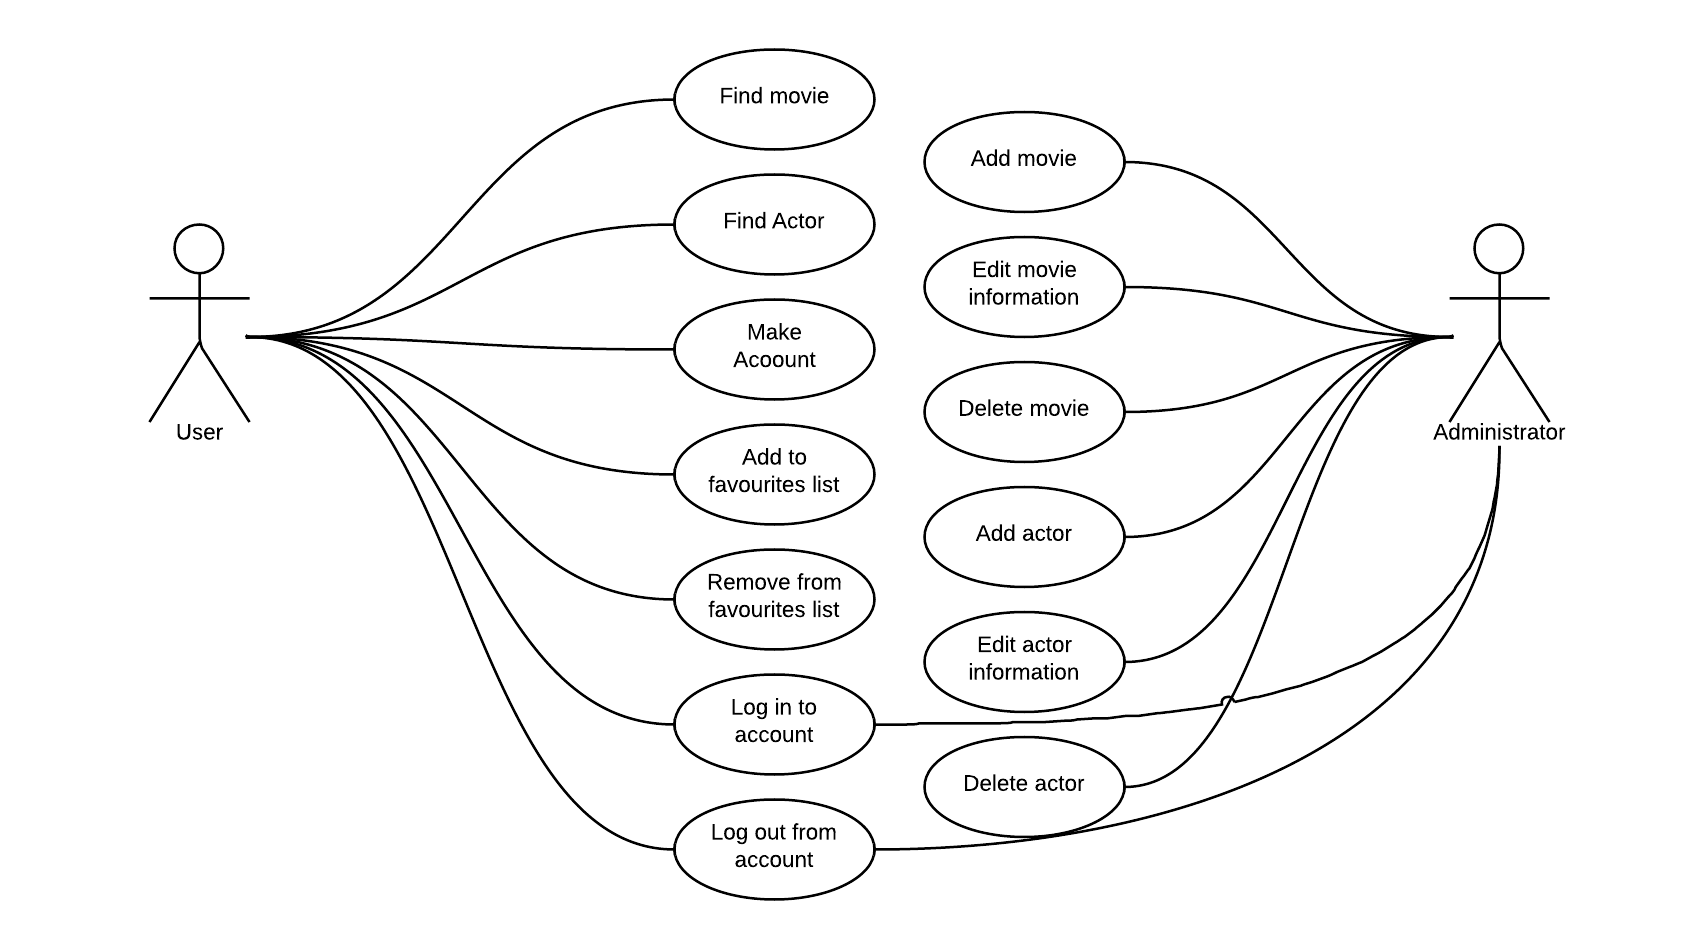
\includegraphics[width=\linewidth]{img/usecasediagram.png}
\caption{Use case diagram}
\label{fig:use case diagram}
\end{figure}

To have a more thorough understanding of each individual use cases, the following explanations was produced, describing each and every step of each use case.
The explanations furthermore include the relation between the actors and the use cases

\begin{center}
	\begin{tabular}{ | l | p{10cm} |  }
		 \hline
		Use Case Name & Find movie \\ \hline
		Participating Actors & Initiated by \emph{User} \\ \hline
		Flow of Events & \begin{enumerate}
						\item[1.] The \emph{user} searches for a movie
						\begin{enumerate}
							\item[2.] The client presents the user with a list of movies with names containing the input
						\end{enumerate}
						\item[3.] The \emph{user} selects one of the search results
						\begin{enumerate}
							\item[4.] The client displays a page containing information on the movie
						\end{enumerate}
					\end{enumerate} \\ \hline
		Entry Condition & \begin{itemize}
						\item The \emph{user} has a client open
					\end{itemize} \\ \hline
		Exit Condition & \begin{itemize}
						\item The \emph{user} successfully found a movie
					\end{itemize} \\
		\hline
	\end{tabular}
\end{center}

\subsection{Defining entity, boundary and control objects}

\subsubsection{Entity objects}

\begin{enumerate}
	\item[1.] Calendar \hfill \\
	A calendar houses a number of events. It has a name and can be part of a 'tag', grouping together calendars
	\item[2.] Event \hfill \\
	An event is the backbone of every calendar. It has a name, description and a date, and must be placed in a specific calendar. Users can add reminders to an event.
	\item[3.] Tag \hfill \\
	A tag is coupled to one or more calendars. By 'tagging' calendars, a user can easily group multiple calendars together.
	\item[4.] Reminder \hfill \\
	A reminder is created along with, or later added to an event. It can be of several types (vibration, email, sound), and will notify the user at a specified time.
\end{enumerate}

\subsubsection{Boundary objects}

\begin{enumerate}
	\item[1.] Device \hfill \\
	The 'device', most likely a smartphone, is our only boundary device, as it houses everything we need to communicate with the user.
\end{enumerate}

\subsubsection{Control objects}

These controllers are all more or less self-explanatory. They enable the user to realise all use cases from their device.

\begin{enumerate}
	\item[1.] MakeEventController
	\item[2.] InspectEventController
	\item[3.] EditEventController 
	\item[4.] DeleteEventController
	\item[5.] InspectCalendarController
	\item[6.] MakeCalendarController
	\item[7.] DeleteCalendarController
	\item[8.] EditCalendarController 
	\item[9.] NotifyUserController 
\end{enumerate}

\subsection{Object model}



\subsection{Dynamic model}



\subsubsection{Sequence diagrams}



\subsubsection{State machines}



\newpage
